%
% This is the LaTeX template file for lecture notes for EE 382C/EE 361C.
%
% To familiarize yourself with this template, the body contains
% some examples of its use.  Look them over.  Then you can
% run LaTeX on this file.  After you have LaTeXed this file then
% you can look over the result either by printing it out with
% dvips or using xdvi.
%
% This template is based on the template for Prof. Sinclair's CS 270.

\documentclass[twoside]{article}
\usepackage{graphics}
\usepackage{tikz}
\usetikzlibrary{arrows}
\usetikzlibrary{decorations.markings,arrows.meta}\tikzset{
arrowmark/.style 2 args={decoration={markings,mark=at     position #1 with \arrow{#2}}}
}
\usepackage{float}
\usepackage{amsmath}
\usepackage[]{algorithm2e}
\usetikzlibrary{arrows,automata}
\usetikzlibrary{arrows,matrix,positioning}
\usepackage[latin1]{inputenc}
\usetikzlibrary{graphs,graphs.standard}
\setlength{\oddsidemargin}{0.25 in}
\setlength{\evensidemargin}{-0.25 in}
\setlength{\topmargin}{-0.6 in}
\setlength{\textwidth}{6.5 in}
\setlength{\textheight}{8.5 in}
\setlength{\headsep}{0.75 in}
\setlength{\parindent}{0 in}
\setlength{\parskip}{0.1 in}
\graphicspath{{images/}}

%
% The following commands set up the lecnum (lecture number)
% counter and make various numbering schemes work relative
% to the lecture number.
%
\newcounter{lecnum}
\renewcommand{\thepage}{\thelecnum-\arabic{page}}
\renewcommand{\thesection}{\thelecnum.\arabic{section}}
\renewcommand{\theequation}{\thelecnum.\arabic{equation}}
\renewcommand{\thefigure}{\thelecnum.\arabic{figure}}
\renewcommand{\thetable}{\thelecnum.\arabic{table}}

%
% The following macro is used to generate the header.
%
\newcommand{\lecture}[4]{
   \pagestyle{myheadings}
   \thispagestyle{plain}
   \newpage
   \setcounter{lecnum}{#1}
   \setcounter{page}{1}
   \noindent
   \begin{center}
   \framebox{
      \vbox{\vspace{2mm}
    \hbox to 6.28in { {\bf EE 382N: Distributed Systems
                        \hfill Fall 2017} }
       \vspace{4mm}
       \hbox to 6.28in { {\Large \hfill Lecture #6: #2  \hfill} }
       \vspace{2mm}
       \hbox to 6.28in { {\it Lecturer: #3 \hfill Scribe: #4} }
      \vspace{2mm}}
   }
   \end{center}
   \markboth{Lecture #1: #2}{Lecture #1: #2}
   %{\bf Disclaimer}: {\it These notes have not been subjected to the
   %usual scrutiny reserved for formal publications.  They may be distributed
   %outside this class only with the permission of the Instructor.}
   \vspace*{4mm}
}

%
% Convention for citations is authors' initials followed by the year.
% For example, to cite a paper by Leighton and Maggs you would type
% \cite{LM89}, and to cite a paper by Strassen you would type \cite{S69}.
% (To avoid bibliography problems, for now we redefine the \cite command.)
% Also commands that create a suitable format for the reference list.
\renewcommand{\cite}[1]{[#1]}
\def\beginrefs{\begin{list}%
        {[\arabic{equation}]}{\usecounter{equation}
         \setlength{\leftmargin}{2.0truecm}\setlength{\labelsep}{0.4truecm}%
         \setlength{\labelwidth}{1.6truecm}}}
\def\endrefs{\end{list}}
\def\bibentry#1{\item[\hbox{[#1]}]}

%Use this command for a figure; it puts a figure in wherever you want it.
%usage: \fig{NUMBER}{SPACE-IN-INCHES}{CAPTION}
\newcommand{\fig}[3]{
			\vspace{#2}
			\begin{center}
			Figure \thelecnum.#1:~#3
			\end{center}
	}
% Use these for theorems, lemmas, proofs, etc.
\newtheorem{theorem}{Theorem}[lecnum]
\newtheorem{lemma}[theorem]{Lemma}
\newtheorem{proposition}[theorem]{Proposition}
\newtheorem{claim}[theorem]{Claim}
\newtheorem{corollary}[theorem]{Corollary}
\newtheorem{definition}[theorem]{Definition}
\newenvironment{proof}{{\bf Proof:}}{\hfill\rule{2mm}{2mm}}

% **** IF YOU WANT TO DEFINE ADDITIONAL MACROS FOR YOURSELF, PUT THEM HERE:

\begin{document}
%FILL IN THE RIGHT INFO.
%\lecture{**LECTURE-NUMBER**}{**DATE**}{**LECTURER**}{**SCRIBE**}
\lecture{1}{October 14}{Vijay Garg}{Samuel Cherinet}
%\footnotetext{These notes are partially based on those of Nigel Mansell.}

% **** YOUR NOTES GO HERE:

% Some general latex examples and examples making use of the
% macros follow.
%**** IN GENERAL, BE BRIEF. LONG SCRIBE NOTES, NO MATTER HOW WELL WRITTEN,
%**** ARE NEVER READ BY ANYBODY.
\section{Leader Election in a Ring}
In distributed systems it is a common occurrence that we want to choose the leader in a network of processes so that the leader could be for example a coordinator of some sort. It is also possible that these processes can have either a unique id or non-unique id. 

\begin{center}
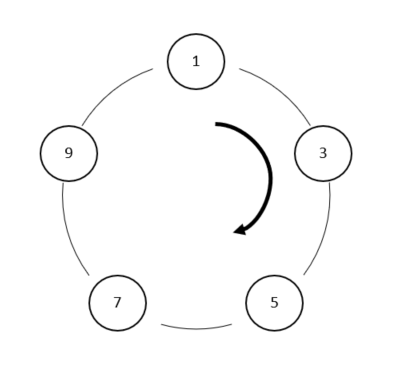
\includegraphics[width=0.5\textwidth]{Ring_diagram_2.png}
\fig{1}{0in}{Simple ring diagram}
\end{center}

So the question is how can we elect a leader? 

There is no deterministic algorithm if the ids are not unique. we can of course randomly pick a leader but there is no deterministic algorithm to pick one. So the assumption ,going forward , is every process has a unique id.And for the sake of simplicity the convention is the process with the biggest id is going to be the leader. the problem is that each of the process doesn't know that he has the biggest number or how many processes there there in the network for that matter.

The algorithm is started by having every process send it's id clockwise to it's left neighbor, algorithm looks much like below:

\begin{algorithm}[H]
 $P_i$::
 
\textbf{var}

\quad{\it myid}: integer;\\
\quad{\it awake}: boolean initally false;\\
\quad{\it leaderid}: integer initally null;\\
\break


To initiate election:\\
\quad send (election,myid) to $P_i_-_1$;\\
\quad awake:=true;\\
\break
Upon receiving a message(election,j):\\
\quad if(j $>$ {\it myid} then\\
\quad\quad send( {\it election, j} ) to P_i_-_1;\\
\quad else if(j = {\it myid}) then\\
\quad\quad send( {\it leader, myid} ) to P_i_-_1;\\
\quad else if((j $<$ {\it myid}) $\wedge$ \neg {\it awake}) then\\
\quad\quad send( {\it election, myid} ) to P_i_-_1;\\
\quad awake:=true;
\newline
Upon receiving a message ({\it leaser,j}):\\
\quad {\it leaderid=j;};\\
\quad if ({\it j=myid}) then {\it send(leader,j)} to P_i_-_1;\\
	
\end{algorithm}

Message Complexity is 
$O(N^2)$
Worst Case Scenario 
$1+2+3+4 ... + N = O(N^2)$

The figure below shows the worst and best cases when determining a ring leader using this algorithm.

\begin{center}
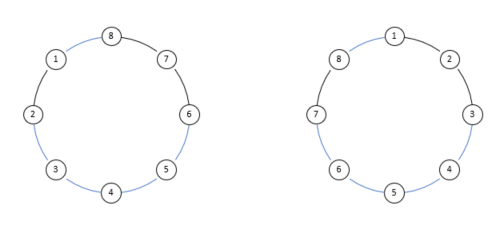
\includegraphics{Ring_diagram_worst_best_case.png}
\fig{2}{0in}{Worst and best case scenarios}
\end{center}

\section{Hierarchical Election}
Now let's try to send message in both directions, then you will not send too many messages. Instead of going around the whole ring, we will use hierarchical election. to be a leader of the ring a process have to be a leader of it's neighborhood. only when a process wins the first round that it can move to the next one.

There is a notion of neighborhood. Let's say d is length of my neighborhood left and right

example 1 left and 1 right, I send a message to both. and with the message I keep the hope count.and the neighbor would only send it back if that guy has a bigger number than you. When you are recipient if your id is smaller than the sender's then you ignore it, since that is a waste of a message. The table below shows the number of messages that are needed as processes go through each round of electing a local leader.

\begin{center}
    \begin{tabular}{| l | l | l | l |}
    \hline
    Round & No. of leaders & d  & No. of messages\\ \hline
    1 & n & 1 & 4n \\ \hline
    2 & n/2 & 2 & 4n \\ \hline
    3 & n/4 & 4 & 4n \\ \hline
    4 & n/8 & 8 & 4n \\ \hline
    .. & .. & .. & .. \\ \hline
    i & i/(2_i_-_1) & (2_i_-_1) & 4n \\ \hline
  
    \hline
    \end{tabular}
    \fig{3}{0in}{Rounds and number of messages it takes}
\end{center}



Number of Messages = O(nlogn)

Theorem
leader election requires \Omega(nlogn)  messages in a ring


\section*{References}
\beginrefs
\bibentry{GARG02}{\sc Vijay K. GARG},
Elements of Distributed Computing,
pp.~163--167.

\endrefs


\end{document}




